% Modificar clase de documento e idiomas, tildes, etc%
\documentclass[twoside, twocolumn, spanish] {article}
\usepackage[spanish,es-tabla]{babel} % tabla
\usepackage[utf8]{inputenc}
\usepackage[export]{adjustbox}
%%%%%%%%%%%%%%%%%%%%%%%%%%%%%%%%%%%%%%%%%%%%%%%%%%%%%%

% Para el enumerate
\usepackage[shortlabels]{enumitem}
\setlength\parindent{0pt}  % quita la indentación
%\setcounter{secnumdepth}{0} % sections are level 1 % para hacer que todas las secciones con* salgan en el índice 


% Paquete y configuración para poder añadir código %
\usepackage{listings}
\usepackage{color} %red, green, blue, yellow, cyan, magenta, black, white
\definecolor{mygreen}{RGB}{28,172,0} 
\definecolor{mylilas}{RGB}{170,55,241}
\definecolor{fondomatlab}{RGB}{255,255,204}
\lstset{language=Matlab,
    %basicstyle=\color{red},
    backgroundcolor=\color{fondomatlab},
    breaklines=true,%
    morekeywords={matlab2tikz},
    keywordstyle=\color{blue},%
    morekeywords=[2]{1}, keywordstyle=[2]{\color{black}},
    identifierstyle=\color{black},%
    stringstyle=\color{mylilas},
    commentstyle=\color{mygreen},%
    showstringspaces=false,%without this there will be a symbol in the places where there is a space
    numbers=left,%
    numberstyle={\tiny \color{black}},% size of the numbers
    numbersep=11pt % this defines how far the numbers are from the text
    emph=[1]{for,end,break},emphstyle=[1]\color{red}, %some words to emphasise
    %emph=[2]{word1,word2}, emphstyle=[2]{style},    
}
%%%%%%%%%%%%%%%%%%%%%%%%%%%%%%%%%%%%%%%%%%%%%%%%%%%%

% valor absoluto y norma
\usepackage{mathtools}
\DeclarePairedDelimiter\abs{\lvert}{\rvert}%
\DeclarePairedDelimiter\norm{\lVert}{\rVert}%

% Paquete circuitikz para dibujar circuitos %
\usepackage{circuitikz}
%%%%%%%%%%%%%%%%%%%%%%%%%%%%%%%%%%%%%%%%%%%%%%%%%%%%%%


% Paquetes de matemáticas %
\usepackage{amsmath,amssymb}
%%%%%%%%%%%%%%%%%%%%%%%%%%%%%%%%%%%%%%%%%%%%%%%%%%%%%%


% Paquetes para cargar gráficos %
\usepackage{graphicx}
\usepackage{subfig}
%%%%%%%%%%%%%%%%%%%%%%%%%%%%%%%%%%%%%%%%%%%%%%%%%%%%%%


% Paquete para hiper enlaces hiperlink %
\usepackage{hyperref}
%%%%%%%%%%%%%%%%%%%%%%%%%%%%%%%%%%%%%%%%%%%%%%%%%%%%%%


% Modificar los márgenes %
\usepackage{geometry}
\geometry{a4paper,hmargin={1.5cm,1.5cm},vmargin={1.5cm,1.5cm}}
\setlength{\columnsep}{0.5cm}
%%%%%%%%%%%%%%%%%%%%%%%%%%%%%%%%%%%%%%%%%%%%%%%%%%%%%%

% Estilo de pagina (cabecera y pie de página)
% Estilo de pagina (cabecera y pie de página)
%\usepackage{fancyhdr}
%\pagestyle{fancy}
%\fancyhf{}   % Reset valores default
	% Para que la sección del encabezado sea la primera que se ve en la pagina
%\renewcommand{\sectionmark}[1]{\markright{#1}{}}
%\fancyhead[CE,CO]{\textsc{\leftmark}}
	% leftmark --> nombre de la última sección de la página
	% CE, CO ---> center even, center odd
	% Otra posible config, con sección a la izda y subsección a la derecha
	% thepage ---> número de página abajo en el centro
%\fancyhead[RE,RO]{\textsc{\rightmark}}
%\fancyhead[LE,LO]{\textsc{\leftmark}}
%\fancyhead[CE,CO]{\textsc{Pongo lo que quiera}}
%\fancyfoot[C]{\thepage}

% \renewcommand{\headrulewidth}{0pt}

%%%%%%%%%%%%%%%%%%%%%%%%%%%%%%%%%%%%%%%%%%%%%%%%%%%%%%

% Paquete para poder añadir código %
\usepackage{listings}
%%%%%%%%%%%%%%%%%%%%%%%%%%%%%%%%%%%%%%%%%%%%%%%%%%%%%%

% Paquete para poder añadir dummy text %
\usepackage{blindtext}
%%%%%%%%%%%%%%%%%%%%%%%%%%%%%%%%%%%%%%%%%%%%%%%%%%%%%%

% Diseño del titulo, resumen y demás %
\usepackage{titling}
\title{Sensobed signal processing using Raspberry Pi\\[0.5cm]	
	\Large{v1.0} \\
}
\author{%
	Mari Carmen Pardo Martínez \\
	\normalsize{Universidad de Granada}\\
	\normalsize{\href{mailto:mcpardo@correo.ugr.es}{mcpardo@correo.ugr.es}}
	\and
	Antonio Javier Pérez Ávila \\
	\normalsize{Universidad de Granada}\\
	\normalsize{\href{mailto:mraeto@correo.ugr.es}{mraeto@correo.ugr.es}}
	}

\date{3 October 2020}
\renewcommand{\maketitlehookd}{

	\renewcommand{\abstractname}{\center{Abstract}}
	\begin{abstract}
This first version of the report broadly covers the work done for the implementation of Sensobed processing in Raspberry Pi.
	\end{abstract}
	\vspace{1cm}
}
%%%%%%%%%%%%%%%%%%%%%%%%%%%%%%%%%%%%%%%%%%%%%%%%%%%%%%%


\begin{document}
\thispagestyle{empty}
\maketitle

\tableofcontents

\section{Introduction}

This project focuses on the sampling and processing of the signals coming from the monitoring system which measures physiological parameters, created in the contract Sensobed2.

\section{Hardware}
In respect of the hardware elements, an ADC converter (ADS1115 by Texas Instruments) and a Raspberry Pi 4 model B.

\begin{itemize}
\item ADS1115: This IC is a 16-bit, I$^2$C-compatible analog-to-digital converter. Its simplified block diagram can be seen in Fig. \ref{ads}. Since it is able to sample bipolar signals, the real resolution for a positive signal is 15 bits. It includes an output pin called ALERT/RDY, which will be configure as RDY in order to generate a positive pulse every time a conversion is ready to be read, as shown in Figure \ref{conversion_ready}.

\begin{figure}[h]
\centering
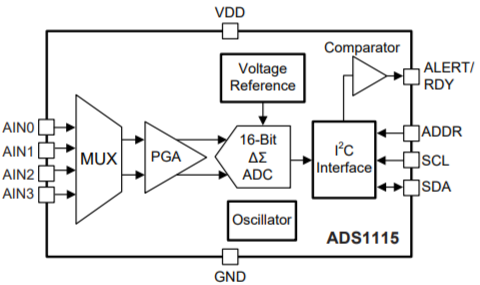
\includegraphics[width=5cm]{imag/ads}
\caption{Simplified block diagram of the ADS1115 ADC converter.}  \label{ads}
\end{figure}

\begin{figure}[h]
\centering
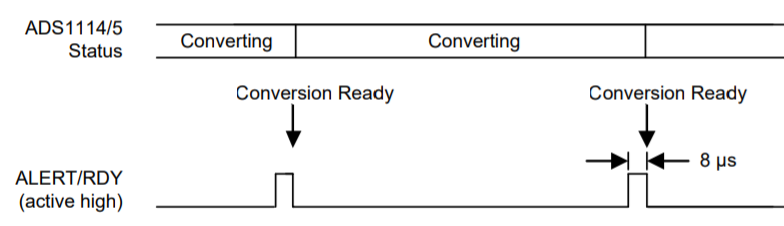
\includegraphics[width=\columnwidth]{imag/conversion_ready_cut}
\caption{Time diagram showing the conversion-ready pulse generated by the ADS1115 when a conversion is completed.}  \label{conversion_ready}
\end{figure}

\item Raspberry Pi 4 Model B: This device is a miniaturized computer which will be in charge of the communication through $I^2C$ protocol with the ADC and of the processing of the transferred samples. Furthermore, the board has communication capabilities such as Bluetooth and Wi-Fi, that will be required later on to sent the results to an Android smartphone.

\end{itemize}  

\section{Firmware}
\subsection{Introduction}
The goal of the firmware is to process the breathing and heart signals in time slots in order to refresh the heart and breathing rate every slot time. Inside of every slot time, two functions appear: the signal sampling and the signal processing, which are required to be concurrent. \\

This idea (shown in Fig. \ref{esquema_general}) is aimed to sample the signal from the measurement system while the processing of the last slot time is being carried out. In a slot, there will be as well a period of time to prepare the next slot, in which the acquired samples are copied to the processing array. A general flowchart of the firmware is shown in Fig. \ref{flowchart_general} for the sake of making this idea as  straightforward as possible. 

\begin{figure}[!h]
\centering
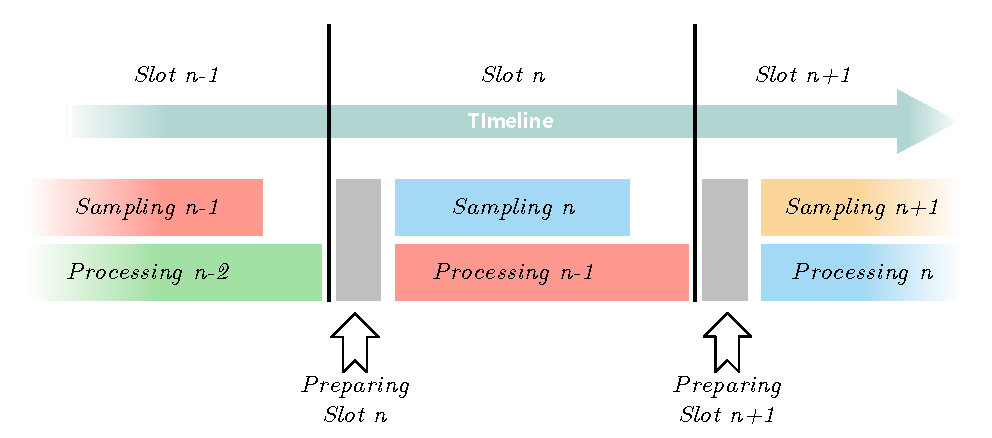
\includegraphics[width=\columnwidth]{imag/esquema_general.pdf}
\caption{General approach of the methodology employed to sample and process the signal.}
\label{esquema_general}
\end{figure}

\begin{itemize}
\item In the initialization, the parameters for the ADC (data rate, gain, $I^2C$ channel) are configured, as well as the variables are declared.
\item After that, there is a loop in which two processes take place simultaneously: sampling of a new group of samples in the slot $n$ and processing of the prior group of samples $n-1$. Both these processes will be described in greater depth in the next section.
\item Only when both of them come to an end, the slot is considered to be finished so that the samples in $n$ move to $n-1$, $n$ is emptied and a new slot is started.
\end{itemize}

\begin{figure}[!h]
\centering
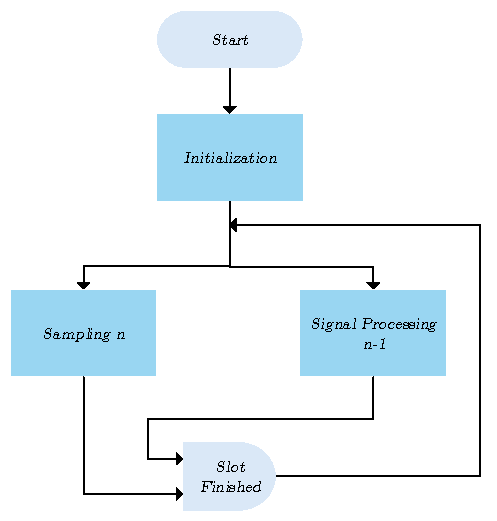
\includegraphics[width=\columnwidth]{imag/flowchart_general}
\caption{Flowchart representing the firmware.}  \label{flowchart_general}
\end{figure}

\subsection{Firmware description}
The program was written in Python 3.8. This section will be focused on the further description of the firmware itself.

\subsubsection{Initialization}
The following Python libraries were used:
\begin{itemize}
\item RPi.GPIO
\item board
\item busio
\item numpy
\item scipy
\item Modified ADS1115 Adrafruit Library
\end{itemize}

The most significant variables declared are the following:
\begin{itemize}
\item $n$: Array where the new samples are storaged.
\item $n\_1$: Array where the samples from the prior time slot are storaged.
\item $slot$: Integer that identifies the time slot.
\item $conv$: Integer that identifies a conversion inside the current
 time slot.
\item $endSampling$: Boolean variable that turns 1 to stop the sampling.
\end{itemize}

Apart from the declaration variables, the initialization also includes the ADC configuration and the definition of an ISR (Interrupt Service Routine). In the sampling section, these will be described with more detail.

\subsubsection{Sampling}
As previously mentioned, sampling was made through the ADC ADS1115. The most relevant parameters used to set up this device (employing a custom modified ADS1115 Adafruit Library) has been the following:
\begin{itemize}
\item ADC object creation: firstly, an ADC object from the mentioned library is defined, indicating the I$^2$C channel. In this definition, the output ALERT/RDY has been configured as RDY. This has required the modification of the Adafruit Library. 
\item Sampling rate: the possible values for this parameter are in the range $[8, 860]$ SPS. The chosen one has been 250 SPS.
\item Conversion mode: contrary to single-shot mode, continuous conversion mode has been enabled in order to let the ADC sample continuously at the stated rate.
\item ADS gain: this ADC has an integrated PGA and it is used to select the correct FSR (Full Scale Range). From the possible values for this parameter, a FSR of $\pm6,144$ V has been picked, which needs the ADS1115 to be supplied with $5$ V.
\end{itemize}


The sampling procedure is drafted on Fig. \ref{flowcharts}b.

\begin{enumerate}
\item Standing up of interuption: first of all, in the slot beginning the bethe interruption is declared and associated with the edge of the signal coming from the output ALERT/RDY of the ADC. Thus, when there is a rising edge in such pin (meaning a conversion is ready) the ISR will be executed.
\item Sample acquisition: inside the ISR, a sample is acquired and added in the $n$ array, which will be processed in the next slot. That way, the $n$ array is gradually filled up.
\item Checking of $n$ array fulfillment.
\item Only when the number of conversions $conv$ reaches the limit imposed $nConv$ (indicating the end of the slot) the end sampling flag $endSampling$ is turned on. Otherwise, $endSampling$ keeps its value on 0, meaning the normal flow of interrruptions will take place.
\end{enumerate}


\begin{figure}[h]
\centering
\subfloat[Flowchart representing the sampling method.]{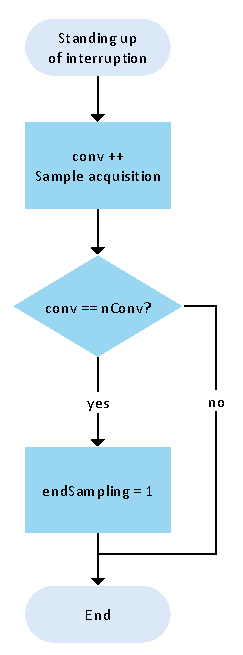
\includegraphics[height=10cm]{imag/flowchart_sampling}} 
\hspace{0.2cm}
\subfloat[Flowchart representing the processing method.]{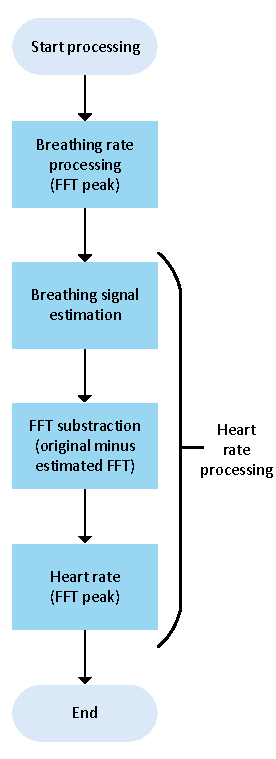
\includegraphics[height=10cm]{imag/flowchart_processing}}
\caption{} 
\label{flowcharts}
\end{figure}

\subsubsection{Processing}
In this section, the processing part of the firmware will be illustrated. The aim of the processing is to obtain heart and breating rates from the samples acquired via the ADC. \\

The starting point for the creation of this process was to generate a signal which would resemble the real signal provided from the sensor as much as possible. For that purpose, real breathing and heart signals (shown in Fig. \ref{starting_signals}a and Fig. \ref{starting_signals}b) have been used. Furthermore, they have been combined and white gaussian noise was added to the resultant signal, as it can be seen in Fig. \ref{combination}. \\

\begin{figure}[h]
\centering
\subfloat[Test breathing signal.]{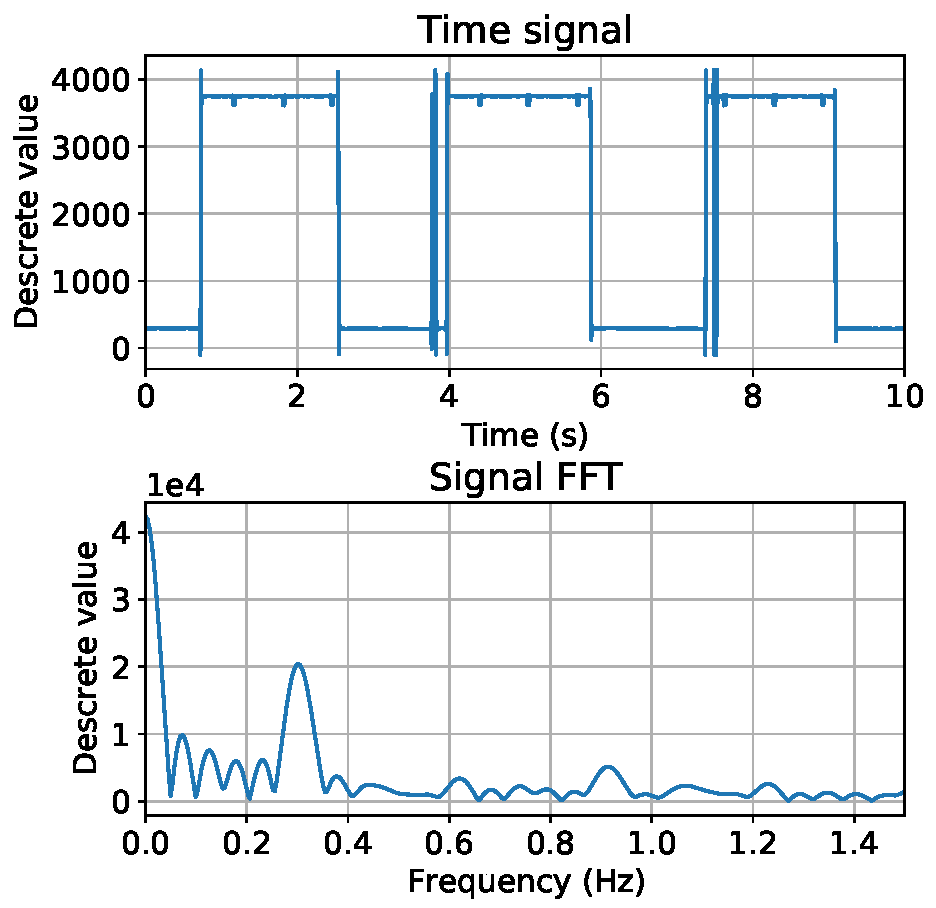
\includegraphics[width=\columnwidth]{imag/proc1}} \\ 
\subfloat[Test heart signal.]{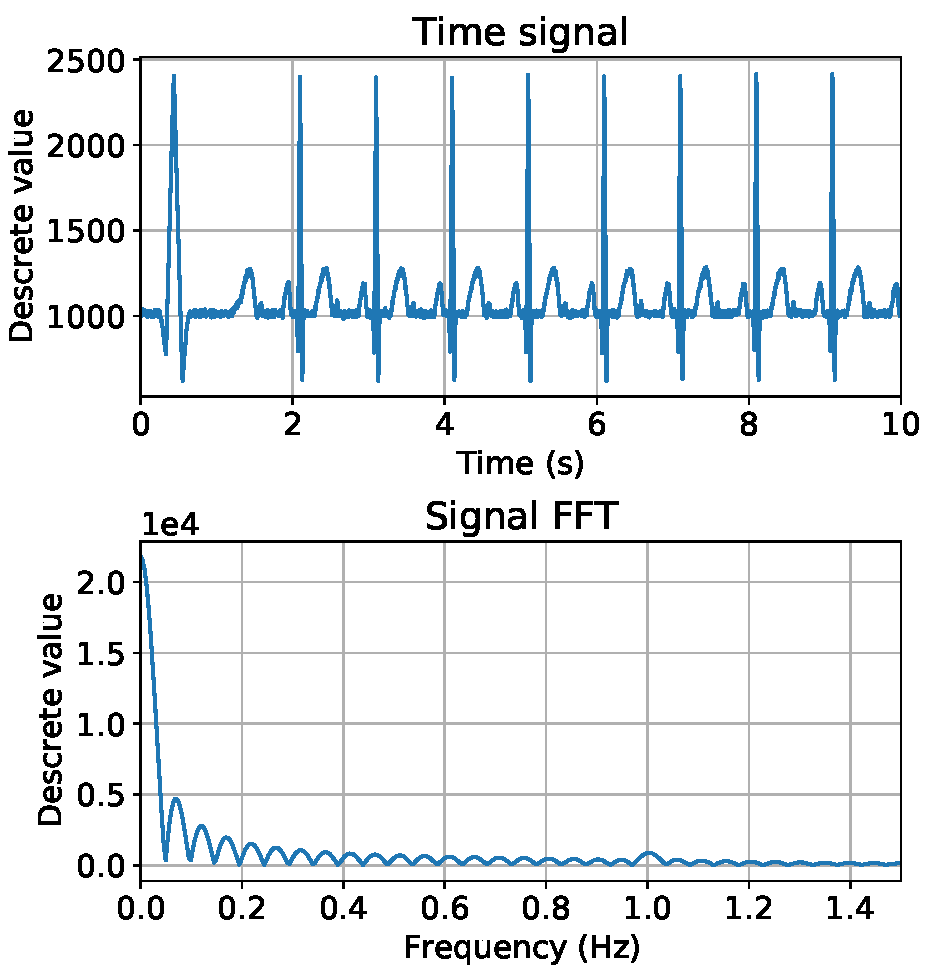
\includegraphics[width=\columnwidth]{imag/proc2}} 
\caption{}
\label{starting_signals}
\end{figure}

\begin{figure}[!h]
\centering
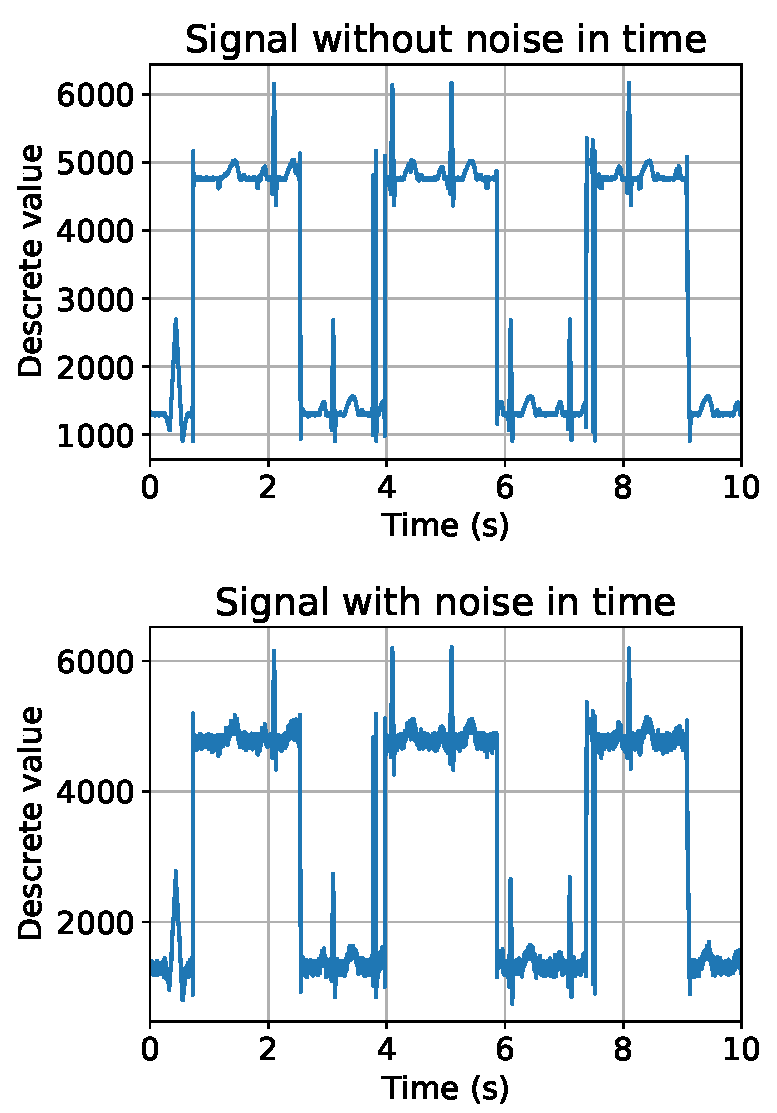
\includegraphics[width=\columnwidth]{imag/proc3}
\caption{Combination of breathing and heart signals, with and without noise.}  \label{combination}
\end{figure}

Once the complete test signal was created, the signal processing showed in Fig. \ref{flowcharts}b is applied to it. 

\begin{enumerate}
\item Breathing rate processing: the signal is filtered with a third order IIR Butterworth band-pass filter made up of SOS (Second Order Section) filters. The upper and lower cutoff frequencies were selected so that the frequencies corresponding to normal breathing rates would not be degraded. As normal sleeping breath rates, the range in $[10,50]$ breaths per minute was taken. Fig. \ref{filter} shows the frequency response of the filter, both in amplitude and phase. By applying this filter to the signal, the result showed in Fig. \ref{filtered_breathing} was achieved.

\begin{figure}[!h]
\centering
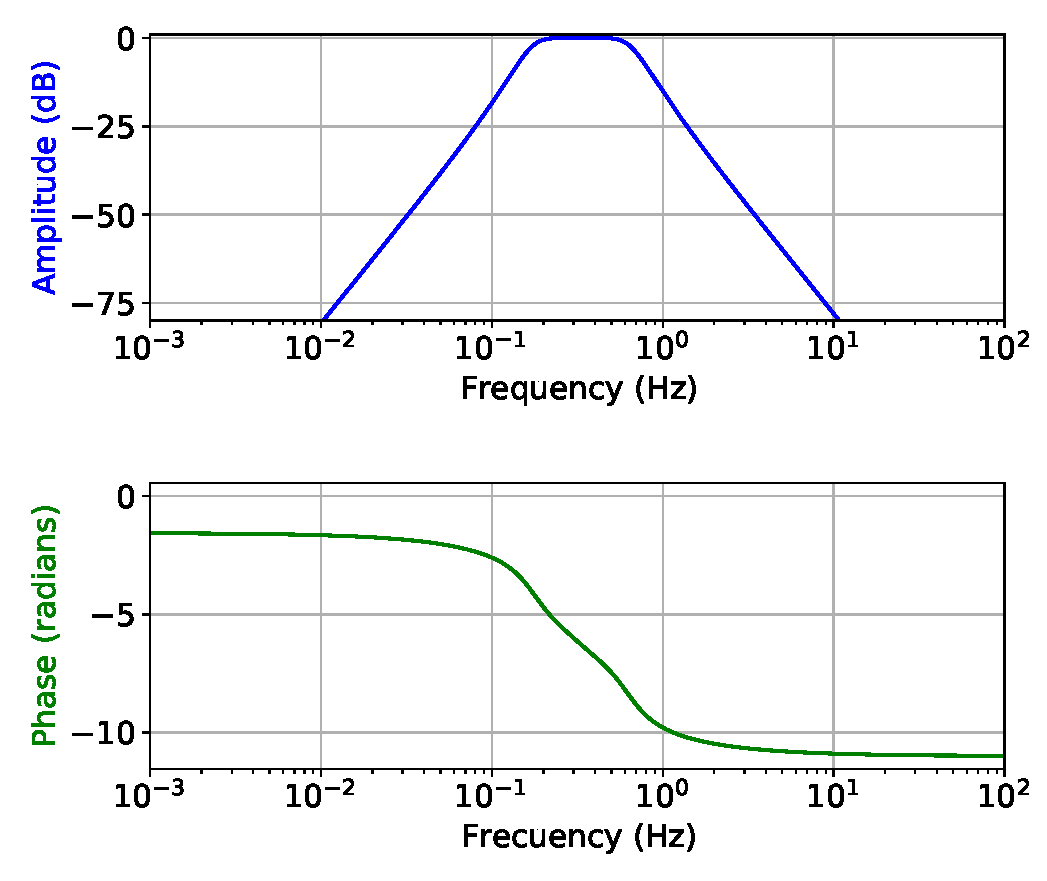
\includegraphics[width=\columnwidth]{imag/proc4}
\caption{Frequency response of the IIR filter for breathing rate obtainment.}  \label{filter}
\end{figure}

%\begin{figure}[!h]
%\centering
%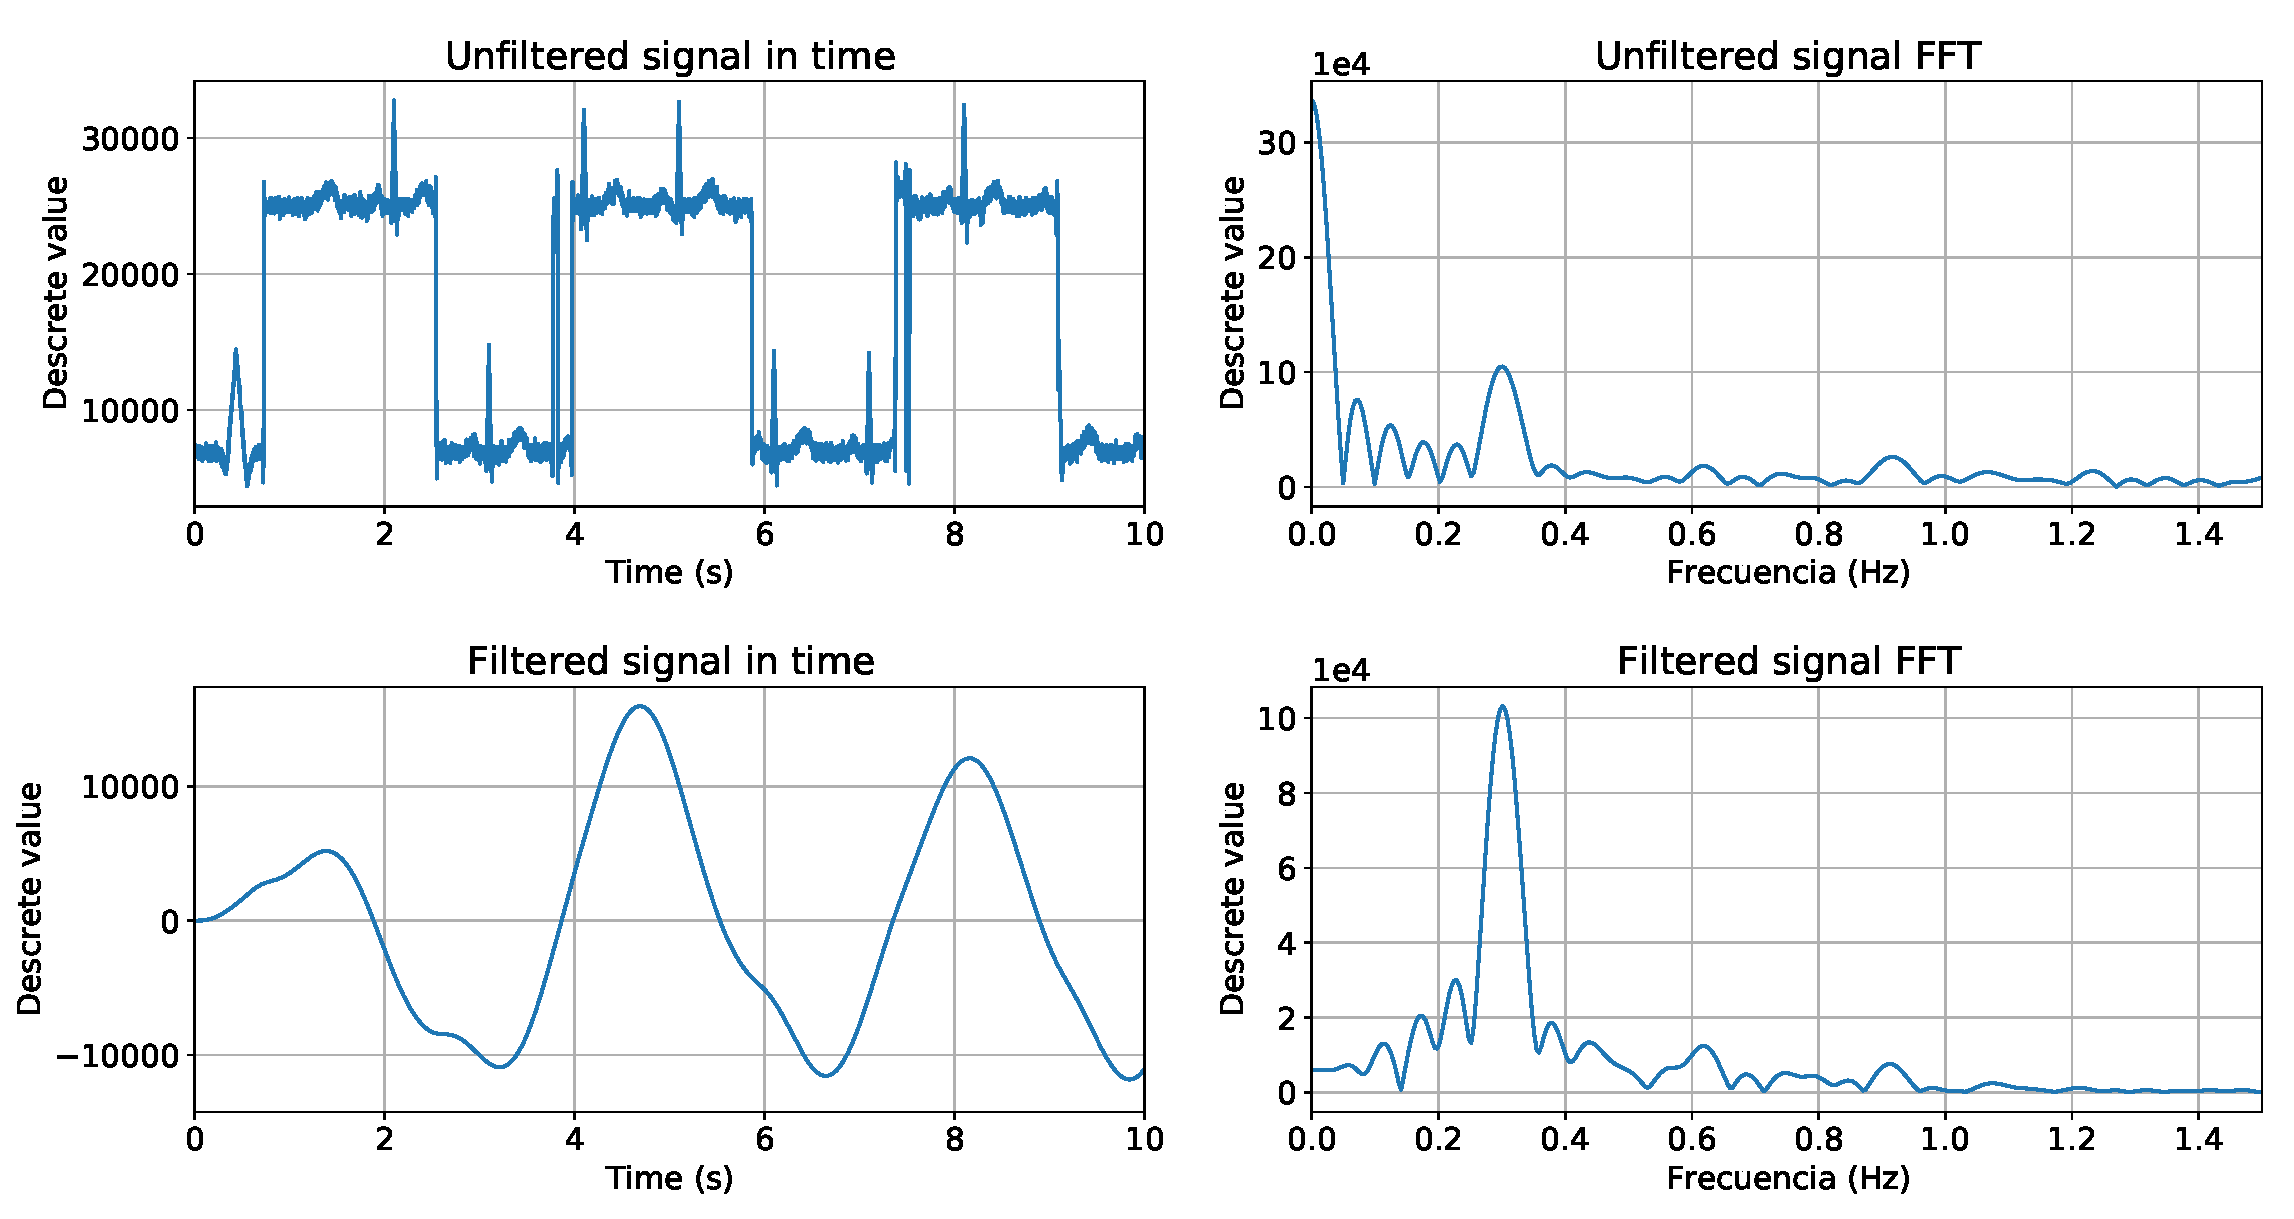
\includegraphics[width=\columnwidth]{imag/proc5}
%\caption{Unfiltered and filtered signals in time and frequency domains.}  \label{filtered_breathing}
%\end{figure}

\begin{figure}[h]
\centering
\subfloat[Unfiltered signal.]{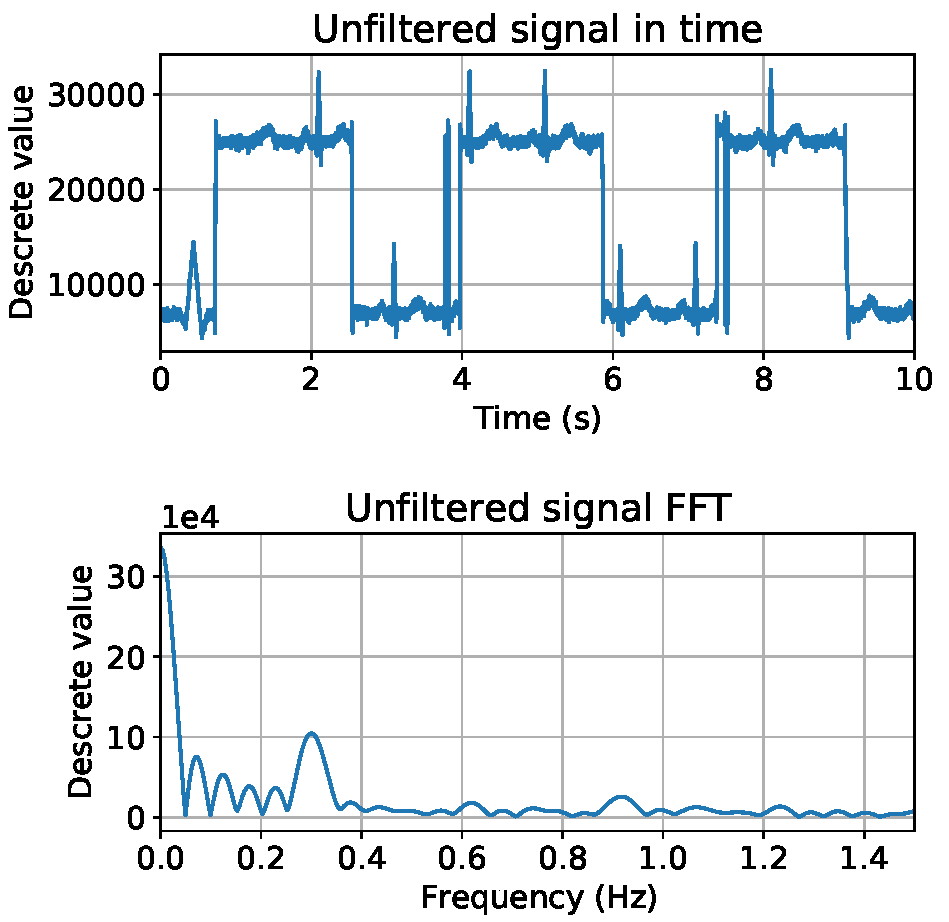
\includegraphics[width=\columnwidth]{imag/proc5a}}  \\
\subfloat[Filtered signal.]{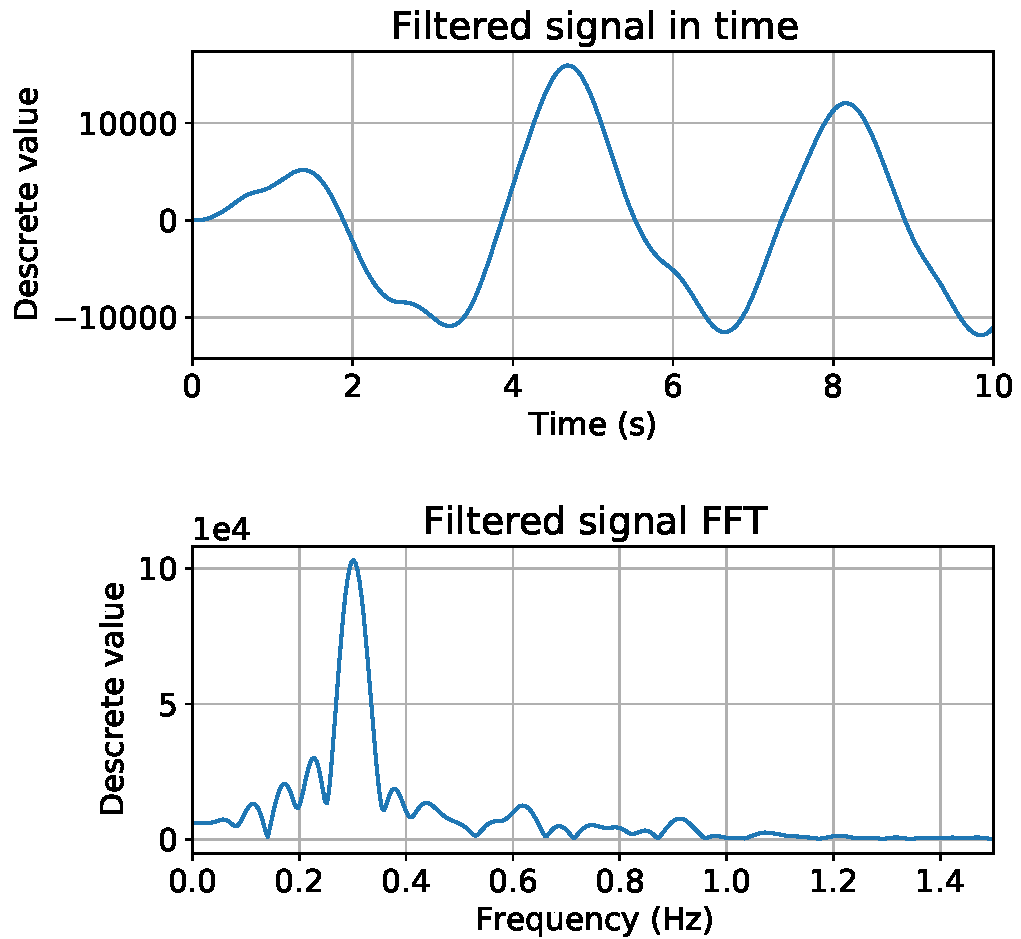
\includegraphics[width=\columnwidth]{imag/proc5b}}
\caption{}
\label{filtered_breathing}
\end{figure}

Subsequently, breath rate was figured out from the filtered signal FFT, where a maximum peak in a specific frequency can be easily detected. From the used signal, the peak is found in $f=0,301$ Hz, which corresponds to a breath rate of $18,082$ Hz.

\item Breathing signal estimation: this is the first step that undertakes heart rate detection. Breathing and heart signals are mixed in the same signal coming from the sensor, being the first much more significant than the second. This fact raised the need to dissociate the two components to obtain the heart rate. 
The method to meet that need was based on the breathing signal estimation: the unfiltered signal in Fig. \ref{filtered_breathing} is separated in two discrete values to compose the typical rectangular breathing shape, resulting in the signal in Fig. \ref{estimation}.

\begin{figure}[!h]
\centering
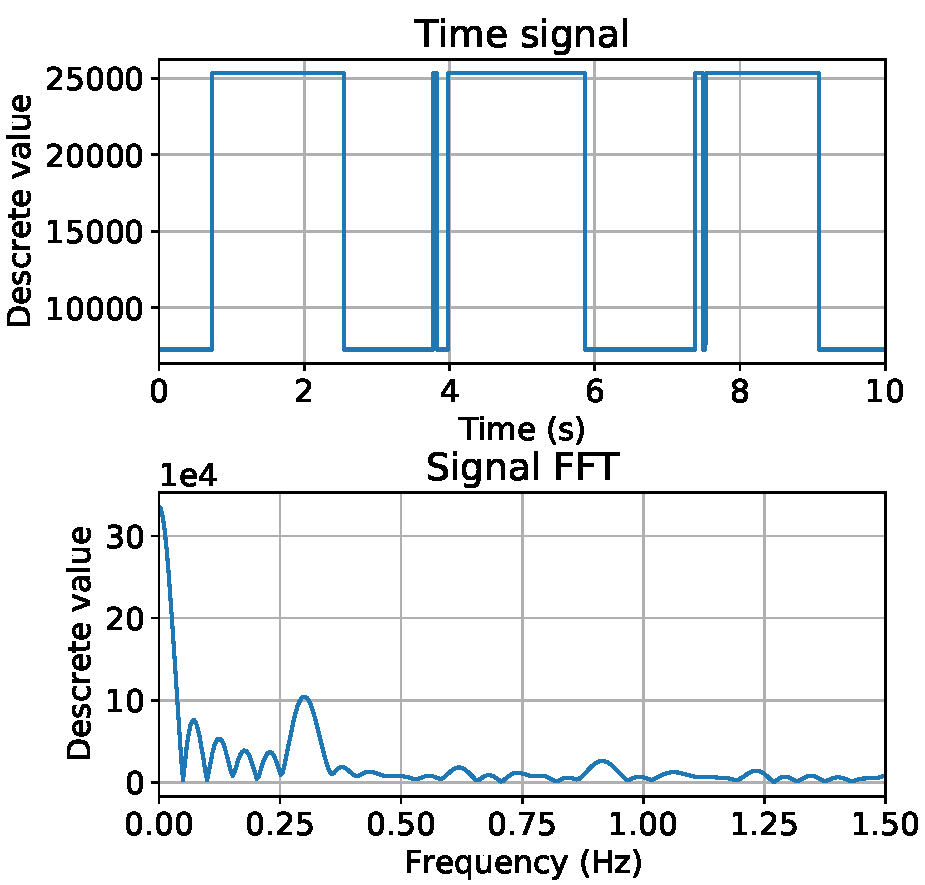
\includegraphics[width=\columnwidth]{imag/proc6}
\caption{Estimated breathing signal in time and frequency domains.}  \label{estimation}
\end{figure}


%\item FFT subtraction: once we have the estimated breathing signal, it is possible to take advantage of the FFT linearity by the subtraction of the estimated breathing signal FFT to the complete signal FFT to obtain an estimated heart signal FFT.
\item FFT subtraction: once the estimated breathing signal is created, it is possible to take advantage of the FFT linearity by the subtraction of the estimated breathing signal FFT to the complete signal FFT to obtain an estimated heart signal FFT.

%to subtract it to the complete signal in order to ontain
\item Heart rate: this frequency can be detected by looking for the maximum peak in the estimated heart signal FFT in the frequency interval between 50 and 200 bpm (Beats Per Minute).
\end{enumerate}

\begin{figure}[!h]
\centering
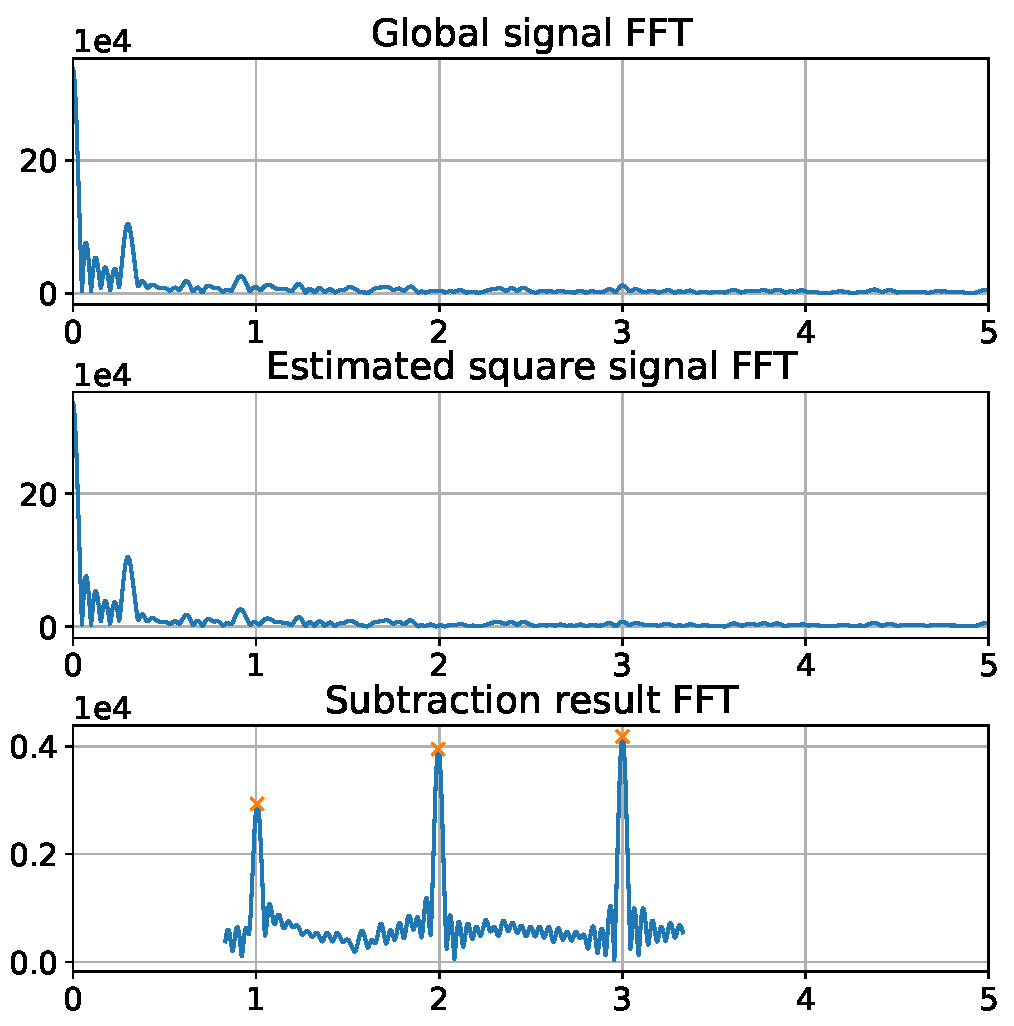
\includegraphics[width=\columnwidth]{imag/proc7}
\caption{Combination of breathing and heart signals, with and without noise.}  \label{heart_rate}
\end{figure}

%
%\begin{figure}[!h]
%\centering
%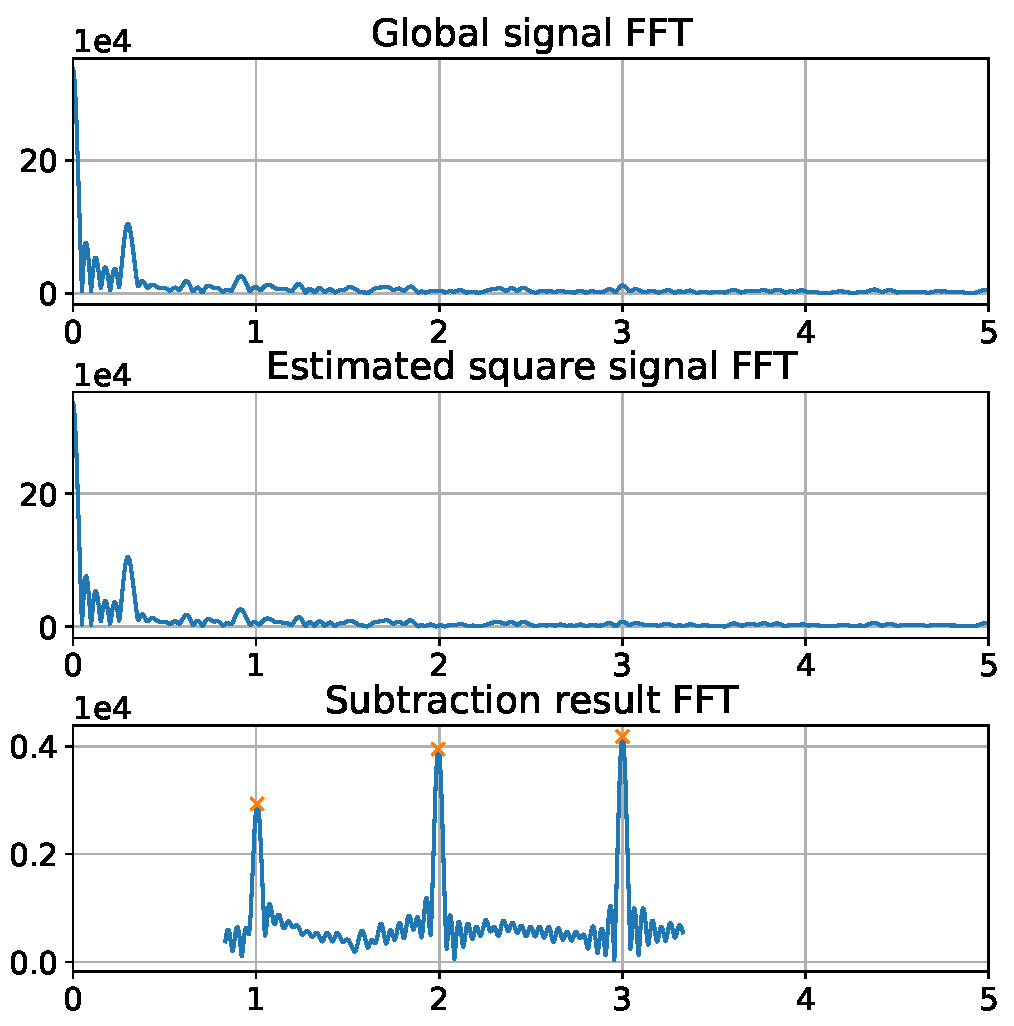
\includegraphics[width=\columnwidth]{imag/proc7}
%\caption{Scheme representing the firmware}  \label{flowchart_general}
%\end{figure}


\subsubsection*{Firmware working conditions}
The commented signal processing works, provided that the breathing signal estimation was similar to the original breathing signal. So, a big heart rate signal (respectively to breathing one) leads to estimation errors, and therefore, non-coherent FFT subtraction. When the heart rate signal increases over a threshold, the estimation is no longer good enough, henceforth the FFT subtraction point is not going to be successful.



\clearpage
%\thispagestyle{fancy}
\end{document}

